\documentclass[11pt,a4paper]{report}
\usepackage[textwidth=37em,vmargin=30mm]{geometry}
\usepackage{calc,xunicode,amsmath,amssymb,paralist,enumitem,tabu,booktabs,datetime2,xeCJK,xeCJKfntef,listings}
\usepackage{tocloft,fancyhdr,tcolorbox,xcolor,graphicx,eso-pic,xltxtra,xelatexemoji}

\newcommand{\envyear}[0]{2024}
\newcommand{\envdatestr}[0]{2024-11-07}
\newcommand{\envfinaldir}[0]{webdb/2024/20241107/final}

\usepackage[hidelinks]{hyperref}
\hypersetup{
    colorlinks=false,
    pdfpagemode=FullScreen,
    pdftitle={Web Digest - \envdatestr}
}

\setlength{\cftbeforechapskip}{10pt}
\renewcommand{\cftchapfont}{\rmfamily\bfseries\large\raggedright}
\setlength{\cftbeforesecskip}{2pt}
\renewcommand{\cftsecfont}{\sffamily\small\raggedright}

\setdefaultleftmargin{2em}{2em}{1em}{1em}{1em}{1em}

\usepackage{xeCJK,xeCJKfntef}
\xeCJKsetup{PunctStyle=plain,RubberPunctSkip=false,CJKglue=\strut\hskip 0pt plus 0.1em minus 0.05em,CJKecglue=\strut\hskip 0.22em plus 0.2em}
\XeTeXlinebreaklocale "zh"
\XeTeXlinebreakskip = 0pt


\setmainfont{Brygada 1918}
\setromanfont{Brygada 1918}
\setsansfont{IBM Plex Sans}
\setmonofont{JetBrains Mono NL}
\setCJKmainfont{Noto Serif CJK SC}
\setCJKromanfont{Noto Serif CJK SC}
\setCJKsansfont{Noto Sans CJK SC}
\setCJKmonofont{Noto Sans CJK SC}

\setlength{\parindent}{0pt}
\setlength{\parskip}{8pt}
\linespread{1.15}

\lstset{
	basicstyle=\ttfamily\footnotesize,
	numbersep=5pt,
	backgroundcolor=\color{black!5},
	showspaces=false,
	showstringspaces=false,
	showtabs=false,
	tabsize=2,
	captionpos=b,
	breaklines=true,
	breakatwhitespace=true,
	breakautoindent=true,
	linewidth=\textwidth
}






\newcommand{\coverpic}[2]{
    % argv: itemurl, authorname
    Cover photo by #2~~(\href{#1}{#1})
}
\newcommand{\makeheader}[0]{
    \begin{titlepage}
        % \newgeometry{hmargin=15mm,tmargin=21mm,bmargin=12mm}
        \begin{center}
            
            \rmfamily\scshape
            \fontspec{BaskervilleF}
            \fontspec{Old Standard}
            \fontsize{59pt}{70pt}\selectfont
            WEB\hfill DIGEST
            
            \vfill
            % \vskip 30pt
            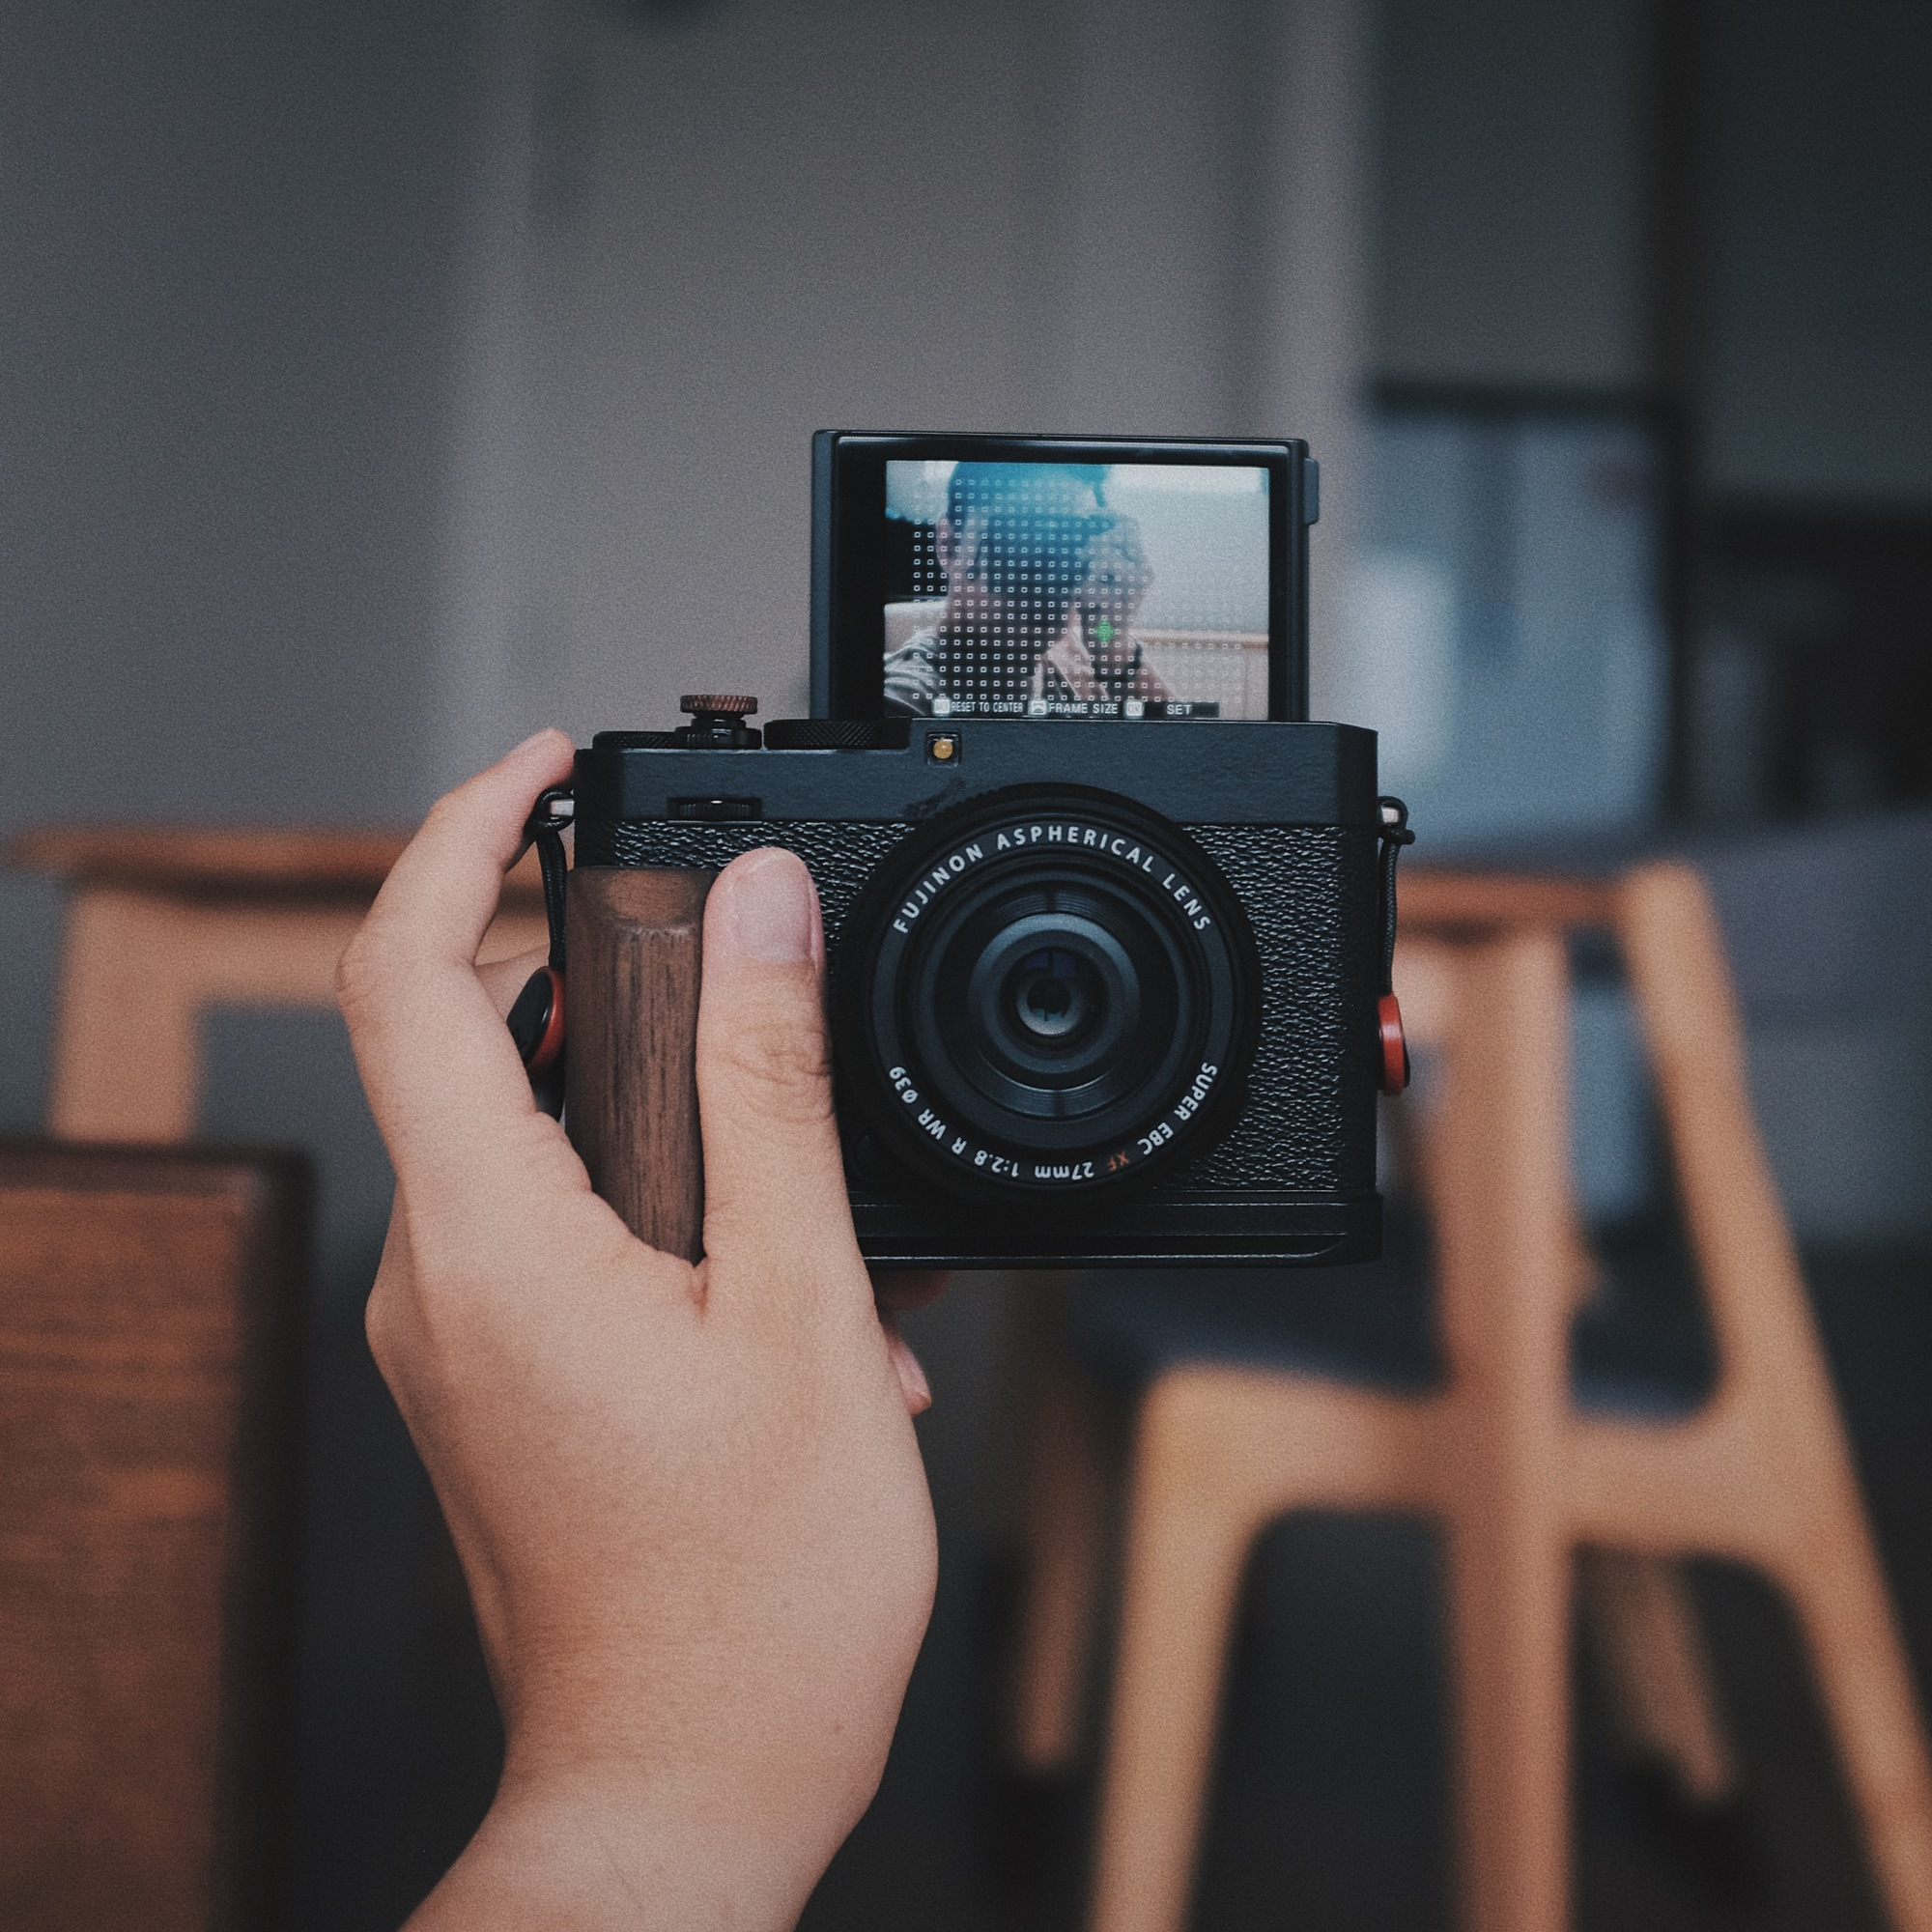
\includegraphics[width=\linewidth]{\envfinaldir/coverpic-prod.jpg}\par
            % \vskip 30pt
            \vfill

            \normalsize\rmfamily\scshape
            \copyright{} The Web Digest Project \hfill\large \envdatestr
        \end{center}
    \end{titlepage}
    % \restoregeometry
}
\newcommand{\simplehref}[1]{%
    \textcolor{blue!80!green}{\href{#1}{#1}}%
}
\renewcommand{\contentsname}{\center\Huge\sffamily\bfseries Contents\par\vskip 20pt}
\newcounter{ipartcounter}
\setcounter{ipartcounter}{0}
\newcommand{\ipart}[1]{
    % \vskip 20pt
    \clearpage
    \stepcounter{ipartcounter}
    \phantomsection
    \addcontentsline{toc}{chapter}{#1}
    % \begin{center}
    %     \Huge
    %     \sffamily\bfseries
    %     #1
    % \end{center}
    % \vskip 20pt plus 7pt
}
\newcounter{ichaptercounter}
\setcounter{ichaptercounter}{0}
\newcommand{\ichapter}[1]{
    % \vskip 20pt
    \clearpage
    \stepcounter{ichaptercounter}
    \phantomsection
    \addcontentsline{toc}{section}{\numberline{\arabic{ichaptercounter}}#1}
    \begin{center}
        \Huge
        \sffamily\bfseries
        #1
    \end{center}
    \vskip 20pt plus 7pt
}
\newcommand{\entrytitlefont}[1]{\subsection*{\raggedright\Large\sffamily\bfseries#1}}
\newcommand{\entryitemGeneric}[2]{
    % argv: title, url
    \parbox{\linewidth}{
        \entrytitlefont{#1}\par\vskip 5pt
        \footnotesize\ttfamily\mdseries
        \simplehref{#2}
    }\vskip 11pt plus 11pt minus 1pt
}
\newcommand{\entryitemGithub}[3]{
    % argv: title, url, desc
    \parbox{\linewidth}{
        \entrytitlefont{#1}\par\vskip 5pt
        \footnotesize\ttfamily\mdseries
        \simplehref{#2}\par\vskip 5pt
        \small\rmfamily\mdseries#3
    }\vskip 11pt plus 11pt minus 1pt
}
\newcommand{\entryitemAp}[3]{
    % argv: title, url, desc
    \parbox{\linewidth}{
        \entrytitlefont{#1}\par\vskip 5pt
        \footnotesize\ttfamily\mdseries
        \simplehref{#2}\par\vskip 5pt
        \small\rmfamily\mdseries#3
    }\vskip 11pt plus 11pt minus 1pt
}
\newcommand{\entryitemHackernews}[3]{
    % argv: title, hnurl, rawurl
    % \parbox{\linewidth}{
    %     \entrytitlefont{#1}\par\vskip 5pt
    %     \footnotesize\ttfamily\mdseries
    %     \simplehref{#3}\par
    %     \textcolor{black!50}{\href{#2}{#2}}
    % }\vskip 11pt plus 11pt minus 1pt
    \begin{minipage}{\linewidth}
            \entrytitlefont{#1}\par\vskip 5pt
            \footnotesize\ttfamily\mdseries
            \simplehref{#3}\par
            \textcolor{black!50}{\href{#2}{#2}}
    \end{minipage}\par\vskip 11pt plus 11pt minus 1pt
}







\begin{document}

\makeheader

\tableofcontents\clearpage




\ipart{Developers}
\ichapter{Hacker News}
\entryitemTwoLinks{Trudeau government bans TikTok from operating in Canada}{https://news.ycombinator.com/item?id=42070946}{https://www.cbc.ca/news/politics/tiktok-canada-review-1.7375965}

\entryitemTwoLinks{Passport Photos}{https://news.ycombinator.com/item?id=42069646}{https://maxsiedentopf.com/passport-photos/}

\entryitemTwoLinks{Caring for yourself while caring for others}{https://news.ycombinator.com/item?id=42068485}{https://magazine.medlineplus.gov/article/caring-for-yourself-while-caring-for-others}

\entryitemTwoLinks{WebSockets cost us \$1M on our AWS bill}{https://news.ycombinator.com/item?id=42067275}{https://www.recall.ai/post/how-websockets-cost-us-1m-on-our-aws-bill}

\entryitemTwoLinks{Starship's Sixth Flight Test}{https://news.ycombinator.com/item?id=42067265}{https://www.spacex.com/launches/mission/?missionId=starship-flight-6}

\entryitemTwoLinks{Learning not to trust the All-In podcast}{https://news.ycombinator.com/item?id=42065538}{https://passingtime.substack.com/p/learning-not-to-trust-the-all-in}

\entryitemTwoLinks{Show HN: Hacker News frontpage as a print newspaper that you can personalize}{https://news.ycombinator.com/item?id=42063709}{https://yourhackernews.com/}

\entryitemTwoLinks{Show HN: Aide, an open-source AI native IDE}{https://news.ycombinator.com/item?id=42063346}{https://aide.dev/}

\entryitemTwoLinks{AMD Ryzen 7 9800X3D Linux Performance: Zen 5 With 3D V-Cache}{https://news.ycombinator.com/item?id=42062934}{https://www.phoronix.com/review/amd-ryzen-7-9800x3d-linux}

\entryitemTwoLinks{Switch 2 will be backwards compatible with Switch}{https://news.ycombinator.com/item?id=42062841}{https://www.videogameschronicle.com/news/nintendo-switchs-successor-will-be-backwards-compatible-with-switch-nintendo-confirms/}

\entryitemTwoLinks{Private Cloud Compute Security Guide}{https://news.ycombinator.com/item?id=42062230}{https://security.apple.com/documentation/private-cloud-compute/}

\entryitemTwoLinks{Bitcoin has made a new all-time high price}{https://news.ycombinator.com/item?id=42062211}{https://www.coinbase.com/price/bitcoin}

\entryitemTwoLinks{Monorepo – Our Experience}{https://news.ycombinator.com/item?id=42062074}{https://ente.io/blog/monorepo-retrospective/}

\entryitemTwoLinks{EU opens antitrust investigation into anticompetitive practices by Corning}{https://news.ycombinator.com/item?id=42061599}{https://ec.europa.eu/commission/presscorner/detail/en/ip\_24\_5681}

\entryitemTwoLinks{What has case distinction but is neither uppercase nor lowercase?}{https://news.ycombinator.com/item?id=42061313}{https://devblogs.microsoft.com/oldnewthing/20241031-00/?p=110443}

\entryitemTwoLinks{Show HN: SuperSplat – open-source 3D Gaussian Splat Editor}{https://news.ycombinator.com/item?id=42060856}{https://playcanvas.com/supersplat/editor?load=https://raw.githubusercontent.com/willeastcott/assets/main/toy-cat.ply\&camera.overlay=false\&show.bound=false}

\entryitemTwoLinks{Show HN: Influencers Database with Audio Signals}{https://news.ycombinator.com/item?id=42058309}{https://old.reddit.com/r/cursor/comments/1gku61m/i\_created\_this\_app\_in\_two\_weekends\_with\_cursor/}

\entryitemTwoLinks{New images of Jupiter}{https://news.ycombinator.com/item?id=42057851}{https://www.missionjuno.swri.edu/junocam/processing?source=all\&ob\_from=2024-10-01\&ob\_to=2024-11-01\&phases\%5B\%5D=PERIJOVE+66\&perpage=16}

\entryitemTwoLinks{Trump wins presidency for second time}{https://news.ycombinator.com/item?id=42057647}{https://thehill.com/homenews/campaign/4969061-trump-wins-presidential-election/}

\entryitemTwoLinks{Useful built-in macOS command-line utilities}{https://news.ycombinator.com/item?id=42057431}{https://weiyen.net/articles/useful-macos-cmd-line-utilities}\ichapter{Phoronix}
\entryitemGeneric{\hskip 0pt{}GIMP 3.2 Will Aim To Be Out Within One Year Of GIMP 3.0}{https://www.phoronix.com/news/GIMP-3.2-One-Year-Goal}

\entryitemGeneric{\hskip 0pt{}Fresh Take On Linux Uncached Buffered I/O "RWF\_UNCACHED" Nets 65~75\% Improvement}{https://www.phoronix.com/news/Linux-RWF\_UNCACHED-2024}

\entryitemGeneric{\hskip 0pt{}systemd 257-rc1 Released With A Ton Of New Features \& Changes}{https://www.phoronix.com/news/systemd-257-rc1}

\entryitemGeneric{\hskip 0pt{}AMD Ryzen 7 9800X3D Linux Performance: Zen 5 With 3D V-Cache}{https://www.phoronix.com/review/amd-ryzen-7-9800x3d-linux}

\entryitemGeneric{\hskip 0pt{}Intel Prepping Linux For SNC6 With Six Nodes Per L3 Cache}{https://www.phoronix.com/news/Intel-Preps-Sub-NUMA-SNC6}

\entryitemGeneric{\hskip 0pt{}Mesa 24.3 Delivers Big Performance Win For Aging AMD Navi 10 GPUs}{https://www.phoronix.com/news/Mesa-24.3-NGG-Culling-RDNA1}

\entryitemGeneric{\hskip 0pt{}Lazy Preemption "PREEMPT\_LAZY" Slated To Land In Linux 6.13}{https://www.phoronix.com/news/Linux-6.13-Lazy-Preemption}

\entryitemGeneric{\hskip 0pt{}cURL 8.11 Released With Official WebSockets Support}{https://www.phoronix.com/news/cURL-8.11-Released}

\entryitemGeneric{\hskip 0pt{}Intel oneCCL 2021.14 Brings New Performance \& Scalability Optimizations}{https://www.phoronix.com/news/Intel-oneCCL-2021.14}


\ipart{Developers~~~~(zh-Hans)}
\ichapter{Solidot}
\entryitemGeneric{\hskip 0pt{}猫脑的衰老与人类相似}{https://www.solidot.org/story?sid=79696}

\entryitemGeneric{\hskip 0pt{}早期黑洞吞噬物质速率超过理论上限的 40 倍}{https://www.solidot.org/story?sid=79695}

\entryitemGeneric{\hskip 0pt{}积极锻炼无法抵消久坐的不良后果}{https://www.solidot.org/story?sid=79694}

\entryitemGeneric{\hskip 0pt{}GIMP 3.0 RC1 开始测试}{https://www.solidot.org/story?sid=79693}

\entryitemGeneric{\hskip 0pt{}世界第一颗木制卫星发射升空}{https://www.solidot.org/story?sid=79692}

\entryitemGeneric{\hskip 0pt{}Google 收到了逾百亿 DMCA 删除请求}{https://www.solidot.org/story?sid=79691}

\entryitemGeneric{\hskip 0pt{}Mozilla 基金会裁员 30\%,关闭倡导和全球项目部门 }{https://www.solidot.org/story?sid=79690}

\entryitemGeneric{\hskip 0pt{}AMD 数据中心业务首次超过英特尔}{https://www.solidot.org/story?sid=79689}

\entryitemGeneric{\hskip 0pt{}长征九号火箭外形类似 SpaceX Starship 的克隆}{https://www.solidot.org/story?sid=79688}

\entryitemGeneric{\hskip 0pt{}当裁决的科学依据被发现是错误的}{https://www.solidot.org/story?sid=79687}

\entryitemGeneric{\hskip 0pt{}Netflix 下架大部分互动剧集}{https://www.solidot.org/story?sid=79686}

\entryitemGeneric{\hskip 0pt{}纽约时报程序员罢工}{https://www.solidot.org/story?sid=79685}

\entryitemGeneric{\hskip 0pt{}FFmpeg 手写 AVX512 汇编代码性能提升最多 94 倍}{https://www.solidot.org/story?sid=79684}

\entryitemGeneric{\hskip 0pt{}洛杉矶县就塑料污染起诉可口可乐和百事可乐}{https://www.solidot.org/story?sid=79683}

\entryitemGeneric{\hskip 0pt{}Meta 核能数据中心受阻于稀有蜜蜂}{https://www.solidot.org/story?sid=79682}

\entryitemGeneric{\hskip 0pt{}莫桑比克在抗议选举后切断移动网络,封禁社交网络}{https://www.solidot.org/story?sid=79681}

\entryitemGeneric{\hskip 0pt{}外星生命能否在无行星环境下生活?}{https://www.solidot.org/story?sid=79680}

\entryitemGeneric{\hskip 0pt{}Meta 在韩国被罚逾 200 亿韩元}{https://www.solidot.org/story?sid=79679}

\entryitemGeneric{\hskip 0pt{}亚马逊 Prime Video 使用 AI 为观众概述正在观看的剧集内容}{https://www.solidot.org/story?sid=79678}

\entryitemGeneric{\hskip 0pt{}粉丝制作《半条命2:第三章》}{https://www.solidot.org/story?sid=79677}\ichapter{V2EX}
\entryitemGeneric{\hskip 0pt{}[问与答] 有没有什么开源的外贸软件}{https://www.v2ex.com/t/1087271}

\entryitemGeneric{\hskip 0pt{}[RSS] 我觉得电脑端 follow 最好用, ios 端 reeder 最好用}{https://www.v2ex.com/t/1087270}

\entryitemGeneric{\hskip 0pt{}[职场话题] 广东真的太热了,不利于创作}{https://www.v2ex.com/t/1087269}

\entryitemGeneric{\hskip 0pt{}[天黑以后] 20241107 午夜俱乐部}{https://www.v2ex.com/t/1087268}

\entryitemGeneric{\hskip 0pt{}[OpenAI] 一個綜合了很多語言模型的在綫 chat,他是怎麽工作的?}{https://www.v2ex.com/t/1087267}

\entryitemGeneric{\hskip 0pt{}[Apple] 求救 iPhone 救砖}{https://www.v2ex.com/t/1087266}

\entryitemGeneric{\hskip 0pt{}[程序员] 现在 8GB 显存 4070 笔记本能训练 AI 画图 LoRA 模型吗?效果怎么样,有没人了解的?我看有的模型说 6GB 显存就能玩}{https://www.v2ex.com/t/1087265}

\entryitemGeneric{\hskip 0pt{}[Python] 帮忙找个历史链接}{https://www.v2ex.com/t/1087264}

\entryitemGeneric{\hskip 0pt{}[问与答] 有哪位老哥知道 Ryzen Master 超频过后应该如何取消吗?}{https://www.v2ex.com/t/1087263}

\entryitemGeneric{\hskip 0pt{}[问与答] 有个外汇相关的问题请教一下}{https://www.v2ex.com/t/1087262}

\entryitemGeneric{\hskip 0pt{}[宽带症候群] Clash(Mihomo)的 DNS 配置可以直接 False 吗?}{https://www.v2ex.com/t/1087261}

\entryitemGeneric{\hskip 0pt{}[分享创造] 做了个完全免费的 AI 音乐生成器,欢迎大家来薅}{https://www.v2ex.com/t/1087260}

\entryitemGeneric{\hskip 0pt{}[杭州] 为了南苕溪钓鱼距离更近 买老余杭比买未科是不是不划算?}{https://www.v2ex.com/t/1087259}

\entryitemGeneric{\hskip 0pt{}[酷工作] 诚邀一位 React 前端大神兼职合作}{https://www.v2ex.com/t/1087257}

\entryitemGeneric{\hskip 0pt{}[程序员] 搞不明白,腾讯是如何把腾讯会议和企业微信接口做的像屎一样的。}{https://www.v2ex.com/t/1087253}

\entryitemGeneric{\hskip 0pt{}[问与答] 我问下有没有日本的朋友用 NAS 的}{https://www.v2ex.com/t/1087250}

\entryitemGeneric{\hskip 0pt{}[宽带症候群] 分别用了电信和联通的 5G 网络进行了测速}{https://www.v2ex.com/t/1087249}

\entryitemGeneric{\hskip 0pt{}[问与答] 坐标江苏,有没有单独开电信宽带比较优惠的方案}{https://www.v2ex.com/t/1087248}

\entryitemGeneric{\hskip 0pt{}[分享发现] FM 上有哪些好的广播和节目推荐一下吗}{https://www.v2ex.com/t/1087247}

\entryitemGeneric{\hskip 0pt{}[Apple] 帮我看看这款 mpb 14 寸 pro 48+512 有没有 国补}{https://www.v2ex.com/t/1087246}

\entryitemGeneric{\hskip 0pt{}[职场话题] 外包和 gap 过久,哪个是 hr 更在意的? V2 的 HR 可以解答下么}{https://www.v2ex.com/t/1087245}

\entryitemGeneric{\hskip 0pt{}[问与答] v 站互联网老哥多,咨询一个很少有人考虑的问题:同一手机号/实名认证,在某 app 注销后再注册,会有记录吗}{https://www.v2ex.com/t/1087244}

\entryitemGeneric{\hskip 0pt{}[职场话题] 去亲戚那里做量化相关工作快两周,来更新一下}{https://www.v2ex.com/t/1087243}

\entryitemGeneric{\hskip 0pt{}[Apple] 要不要出手 mac mini m4 pro 24G+512G(国补后 8999)?}{https://www.v2ex.com/t/1087242}

\entryitemGeneric{\hskip 0pt{}[Amazon Web Services] AWS 1v-8v-32v-谁能告诉我?}{https://www.v2ex.com/t/1087239}

\entryitemGeneric{\hskip 0pt{}[Vue.js] 有没有像 freecodecamp.org 这样的网站?}{https://www.v2ex.com/t/1087238}

\entryitemGeneric{\hskip 0pt{}[问与答] 兄弟们指点一下我这种情况我还应该继续吗}{https://www.v2ex.com/t/1087237}

\entryitemGeneric{\hskip 0pt{}[上海] 上海近一号线锦江乐园站房东整租一室一厅}{https://www.v2ex.com/t/1087236}

\entryitemGeneric{\hskip 0pt{}[Ruby] 有对 Ruby 感兴趣的吗?}{https://www.v2ex.com/t/1087235}

\entryitemGeneric{\hskip 0pt{}[职场话题] 大家骑驴找马的时候是咋沟通线下面试的}{https://www.v2ex.com/t/1087233}

\entryitemGeneric{\hskip 0pt{}[宽带症候群] 广东移动现在变成 nat4, bt 跑不了, p2p 联机的游戏都玩不了}{https://www.v2ex.com/t/1087229}

\entryitemGeneric{\hskip 0pt{}[推广] 阿里云特价服务器 7 折入口,亲测可行}{https://www.v2ex.com/t/1087228}

\entryitemGeneric{\hskip 0pt{}[游戏] 有喜欢龙珠的朋友吗?等待 17 年的电光炸裂 ZERO 出了,做了个视频有挺多讨论}{https://www.v2ex.com/t/1087227}

\entryitemGeneric{\hskip 0pt{}[问与答] Mac 上如何使用 GUI 自动化/RPA 批量导出剪映草稿?}{https://www.v2ex.com/t/1087226}

\entryitemGeneric{\hskip 0pt{}[Android] 5 年小米/红米用户,准备换新手机,问下其他厂商有啥推荐的}{https://www.v2ex.com/t/1087225}

\entryitemGeneric{\hskip 0pt{}[分享发现] 分享一个程序员都可以试试的短视频实践}{https://www.v2ex.com/t/1087224}

\entryitemGeneric{\hskip 0pt{}[问与答] 求推荐一个机架式服务器}{https://www.v2ex.com/t/1087223}

\entryitemGeneric{\hskip 0pt{}[分享发现] 现在各手机厂商的主打手机怎么越来越贵了?}{https://www.v2ex.com/t/1087222}

\entryitemGeneric{\hskip 0pt{}[iOS] [Bug] iOS18.2 Beta 查找无法具体定位 Airtag 和 AirPods Pro 2}{https://www.v2ex.com/t/1087220}

\entryitemGeneric{\hskip 0pt{}[投资] 懂王上台了,比特币新高了,特斯拉股票盘前涨了 14\%, 288 了。}{https://www.v2ex.com/t/1087219}

\entryitemGeneric{\hskip 0pt{}[macOS] mac 照片应用编辑图片后报错}{https://www.v2ex.com/t/1087218}

\entryitemGeneric{\hskip 0pt{}[问与答] 成年人只做筛选, 不教育是否应用于家人(长辈)?}{https://www.v2ex.com/t/1087217}

\entryitemGeneric{\hskip 0pt{}[Mac mini] Mac mini m4 首发前几天可以直接在直营店买到吗}{https://www.v2ex.com/t/1087216}

\entryitemGeneric{\hskip 0pt{}[NAS] 北京联通还是可以的?能做到双栈公网 IP + 便宜 100M 大上行}{https://www.v2ex.com/t/1087215}

\entryitemGeneric{\hskip 0pt{}[分享发现] 刚剁手的三星 g8 oled 玩了一下午,感觉眼睛挺累的}{https://www.v2ex.com/t/1087214}

\entryitemGeneric{\hskip 0pt{}[Telegram] telegram 有没有什么好用安全的第三方客户端(Android)?}{https://www.v2ex.com/t/1087213}

\entryitemGeneric{\hskip 0pt{}[Android] Magisk 如何给别的机器修补 boot.img}{https://www.v2ex.com/t/1087211}

\entryitemGeneric{\hskip 0pt{}[Visual Studio Code] Vscode 里, terminal 里,我开了两个终端(通过点击+号 新增的终端),怎么切换呀?}{https://www.v2ex.com/t/1087210}

\entryitemGeneric{\hskip 0pt{}[酷工作] 赴日开发大量要人!日本 N3 以上,急求!}{https://www.v2ex.com/t/1087207}

\entryitemGeneric{\hskip 0pt{}[宽带症候群] 上海电信疑似给境外流量限流}{https://www.v2ex.com/t/1087206}


\ipart{Generic News}
\ichapter{AP News}
\entryitemWithDescription{\hskip 0pt{}Rapper Tekashi 6ix9ine strikes deal to end jail stint}{https://apnews.com/article/fa363bd39c7a115494f0575aed37c79c}{}

\entryitemWithDescription{\hskip 0pt{}UK doctor gets 31 years for poisoning mother's partner with fake COVID vaccine}{https://apnews.com/article/ffc3a2fbdf8c27a561cf6d39e0525611}{}

\entryitemWithDescription{\hskip 0pt{}Tesla shares soar more than 14\% as Trump win is seen boosting Elon Musk's electric vehicle company}{https://apnews.com/article/b54454aaabd4cbe1e1e1c9754649b869}{}

\entryitemWithDescription{\hskip 0pt{}The first car made during Soviet-era in Poland goes on display 73 years later}{https://apnews.com/article/b821f6b848d2295dbb0c15c84027f326}{}

\entryitemWithDescription{\hskip 0pt{}Hurricane Rafael makes landfall in Cuba as a Category 3 storm after knocking out power on the island}{https://apnews.com/article/f96033ae40b18d745f95d9dd17868457}{}

\entryitemWithDescription{\hskip 0pt{}Record-high pollution sickens thousands in Pakistan's cultural capital of Lahore}{https://apnews.com/article/3bada25447094a3b1bd62d3be38b5984}{}

\entryitemWithDescription{\hskip 0pt{}It's not official yet but Mount Fuji gets its trademark snowcap after the longest delay in 130 years}{https://apnews.com/article/82e3918efb149a5caf7865eca3c8baf8}{}

\entryitemWithDescription{\hskip 0pt{}Woman accusing Conor McGregor of sexual assault testifies in court at start of civil case}{https://apnews.com/article/c8bc44ad320846af9c64024d6615042f}{}

\entryitemWithDescription{\hskip 0pt{}Dodgers star Shohei Ohtani has surgery to repair labrum tear in shoulder after World Series injury}{https://apnews.com/article/74a9dd825e15cd5a11dabbd94baf3734}{}

\entryitemWithDescription{\hskip 0pt{}The world watches as US election results trickle in}{https://apnews.com/article/61fcafce34fffca9647e4616e0159c0c}{}

\entryitemWithDescription{\hskip 0pt{}Influencer is banned from future NYC marathons for bringing a camera crew to last weekend's race}{https://apnews.com/article/11d6d04fda7826bab3d8f263750ecefd}{}

\entryitemWithDescription{\hskip 0pt{}Ruby slippers from `The Wizard of Oz' are for sale nearly 2 decades after they were stolen}{https://apnews.com/article/96f32011bac9d8b55432079c3f91f9d5}{}

\entryitemWithDescription{\hskip 0pt{}Home Depot's co-founder and billionaire philanthropist dies at 95}{https://apnews.com/article/67e518764bcdbe549d369d2297058c28}{}\ichapter{Reuters}
\entryitemWithDescription{\hskip 0pt{}Kamala Harris concedes election to Trump but vows to fight on}{https://www.reuters.com/world/us/kamala-harris-concedes-election-vows-fight-2024-11-06/}{U.S. Vice President Kamala Harris delivered a concession speech to the nation on Wednesday after a whirlwind campaign that failed to stop Republican Donald Trump\textquotesingle s return to the White...}

\entryitemWithDescription{\hskip 0pt{}UK PM Starmer speaks with Donald Trump to offer "hearty congratulations"}{https://www.reuters.com/world/uk-pm-starmer-speaks-with-donald-trump-offer-hearty-congratulations-2024-11-06/}{British Prime Minister Keir Starmer spoke with U.S. President-elect Donald Trump on Wednesday to congratulate Trump on his election...}

\entryitemWithDescription{\hskip 0pt{}Panama to cancel flags on four US-sanctioned LNG vessels}{https://www.reuters.com/world/americas/panama-cancel-flags-four-us-sanctioned-lng-vessels-2024-11-06/}{Panama\textquotesingle s Maritime Authority said on Wednesday it has begun a process to cancel flag registrations on four LNG vessels sanctioned by the United States over their links with Russian gas producer...}

\entryitemWithDescription{\hskip 0pt{}Trump's return to power fueled by Hispanic, working-class voter support}{https://www.reuters.com/world/us/trumps-return-power-fueled-by-hispanic-working-class-voter-support-2024-11-06/}{Donald Trump reshaped the U.S. electorate once again this year, piling up support among Hispanic voters, young people, and Americans without college degrees -\/- and winning more votes in nearly all of the country as he reclaimed the...}

\entryitemWithDescription{\hskip 0pt{}Germany's Scholz to call confidence vote, sees snap election in March}{https://www.reuters.com/world/europe/germanys-scholz-call-confidence-vote-sees-snap-election-march-2024-11-06/}{German Chancellor Olaf Scholz said on Wednesday he would call a confidence vote on January 15, which could pave the way for a snap federal election in...}

\entryitemWithDescription{\hskip 0pt{}White House plans to rush military aid to Ukraine by inauguration day, Politico reports}{https://www.reuters.com/world/white-house-plans-rush-military-aid-ukraine-by-inauguration-day-politico-reports-2024-11-06/}{The White House is planning to rush the last of over \$6 billion remaining in Ukraine security assistance out the door by the time President-elect Donald Trump takes office, Politico reported on Wednesday, citing two Biden administration...}

\entryitemWithDescription{\hskip 0pt{}Biden congratulates Trump, invites him to White House}{https://www.reuters.com/world/us/biden-congratulates-trump-invites-him-white-house-2024-11-06/}{Democratic U.S. President Joe Biden on Wednesday called to congratulate Donald Trump on his presidential election victory and invite him to meet at the White House and will address the nation on...}

\entryitemWithDescription{\hskip 0pt{}German Chancellor Scholz sacks finance minister over budget dispute, sources say}{https://www.reuters.com/world/europe/german-chancellor-scholz-sacks-finance-minister-over-budget-dispute-sources-say-2024-11-06/}{German Chancellor Olaf Scholz sacked his Finance Minister Christian Lindner on Wednesday after weeks of wrangling over the future economic direction of the government, two sources told...}

\entryitemWithDescription{\hskip 0pt{}Harris called Trump to concede US presidential election, aides say}{https://www.reuters.com/world/us/harris-called-trump-concede-us-presidential-election-aides-say-2024-11-06/}{Democratic Vice President Kamala Harris called Donald Trump on Wednesday to congratulate the Republican leader on his U.S. presidential election win, two aides to Harris...}

\entryitemWithDescription{\hskip 0pt{}Trump's victory adds to Trudeau's challenges in Canada}{https://www.reuters.com/world/americas/trumps-victory-adds-trudeaus-challenges-canada-2024-11-06/}{Donald Trump\textquotesingle s return to the White House next year could bring economic pain and difficult decisions for Canada\textquotesingle s Liberal Prime Minister Justin Trudeau, once branded a "far left lunatic" by the...}

\entryitemWithDescription{\hskip 0pt{}US expands sanctions against Bosnian Serb leader's network}{https://www.reuters.com/world/us-expands-sanctions-against-bosnian-serb-leaders-network-2024-11-06/}{The United States on Wednesday expanded sanctions against an individual and an entity who have helped Bosnian Serb nationalist leader Milorad Dodik and his son evade existing U.S. sanctions, the U.S. Treasury Department said in a...}

\entryitemWithDescription{\hskip 0pt{}UN to Israel: Replacing UNRWA relief agency would be your responsibility}{https://www.reuters.com/world/un-signals-israel-replacing-unrwa-would-be-your-responsibility-2024-11-06/}{The U.N. formally responded in a letter to Israel\textquotesingle s decision to sever ties with the United Nations Relief and Works Agency, a move UNRWA says risks collapsing its operations in Gaza and the West...}

\entryitemWithDescription{\hskip 0pt{}Trump could harden Iran oil stance but struggle to stem flow to China, analysts say}{https://www.reuters.com/business/energy/trump-could-harden-iran-oil-stand-raise-china-ire-analysts-say-2024-11-06/}{Former President Donald Trump\textquotesingle s return to the White House could mean tougher enforcement of U.S. oil sanctions against Iran, potentially trimming global supplies, but his administration could struggle to get China, Iran...}\ichapter{联合早报}
\entryitemWithDescription{沈泽玮:台湾冲突阻遏法案只叫不咬?}{https://www.zaobao.com/news/china/story20240918-4758889}{美国众议院9月9日开启了长达一星期的``中国周'',共通过25项主要涉华法案。(法新社) 美国众议院在当地时间9月9日开启了长达一星期的``中国周'',在美国总统和国会选举举行之前,密集表决数十项与中国有关的法案,共通过25项主要涉华法案……}

\entryitemWithDescription{欧盟电动车关税投票倒计时 中国在分歧中寻支持}{https://www.zaobao.com/news/china/story20240917-4758953}{欧盟27个成员国将于9月25日就是否继续对进口自中国的电动汽车额外征税进行最后表决。图为上海港等待装运出口的电动汽车。(彭博社) 欧盟对中国电动汽车加征关税的投票进入倒计时,正在欧洲访问的中国商务部部长王文涛与欧盟多国政府高层就此进行协商,试图在立场分歧的成员国中争取到更多支持。 受访学者研判,欧盟对中国电动汽车加征关税不可避免,但具体的加税方式和幅度仍有一定弹性,这是王文涛此行与各国谈判的重点……}

\entryitemWithDescription{港府今年将举办逾400项国庆活动}{https://www.zaobao.com/news/china/story20240917-4759341}{再过十多天就是中国国庆75周年,香港天星小轮展示``国庆75周年''\,``三天免费搭小轮''等标语迎国庆。(中新社) 再过十多天就是中国国庆75周年,香港特区政府今年将举办逾400项庆祝活动,希望通过一连串活动庆祝国庆,并且弘扬爱国主义教育及刺激消费。 港府星期二(9月17日)召开记者会,介绍各项庆祝国庆活动和特别优惠,涉及出行及吃喝玩乐等领域……}

\entryitemWithDescription{美空军部长:中国大陆军演精密化 为入侵封锁台湾做准备}{https://www.zaobao.com/news/china/story20240917-4759407}{美国空军部长肯德尔星期一(9月16日)在空军暨太空军协会的一场大会上致辞,提到中国对印太地区日益增长的威胁。(取自美国国防部网站) (华盛顿综合讯)美国空军部长肯德尔指,中国大陆军演的规模越来越大,也更加精密化,这是在专门为入侵、封锁台湾做准备。他也称,中国对印太地区的威胁现在已存在……}

\entryitemWithDescription{批准潜在对台备件军售案后 美派巡逻机过航台海}{https://www.zaobao.com/news/china/story20240917-4758770}{台军士兵8月26日在屏东县枋山训练场进行实弹演习时,从M1167 TOW运载车上发射一枚美制TOW-2A线导反坦克导弹。(路透社) (华盛顿/台北/北京综合讯)在批准潜在对台备件军售案之后,美国派遣反潜巡逻机过航台湾海峡,中国人民解放军东部战区则组织战机跟监美机,并誓言``坚决捍卫国家主权''……}

\entryitemWithDescription{李家超:若香港驻美经贸办被关 受害的是美企}{https://www.zaobao.com/news/china/story20240917-4758797}{香港特首李家超星期一(9月17日)警告,如果美国通过法案,导致香港驻美经贸办关闭,受害的是美国企业。图为李家超9月11日在``一带一路''高峰论坛上致辞。(彭博社) (香港综合讯)香港特首李家超警告,如果美国通过法案,导致香港驻美经贸办关闭,受害的是美国企业。 美国众议院上周通过《香港经济贸易办事处认证法案》,如果参议院也表决通过并交由总统签署成法,香港三个驻美国的经贸办可能将被强制关闭……}

\entryitemWithDescription{美国指中国航空工业集团员工企图实施黑客攻击}{https://www.zaobao.com/news/china/story20240917-4757988}{(华盛顿综合讯)中国航空航天巨头中国航空工业集团一名员工被指试图对美国宇航局、美国军方和其他目标展开黑客攻击。 据彭博社报道,美国检察官布坎南星期一(9月16日)在起诉书中,指控中国航空工业集团39岁的工程师吴宋(音译,Song Wu)企图从美国宇航局、空军、陆军和海军,以及联邦航空管理局取得电脑软件和源代码……}

\entryitemWithDescription{【东谈西论】恒大账务造假 普华永道是共犯还是被拖累?}{https://www.zaobao.com/news/china/story20240917-4756452}{因涉及恒大地产审计项目的违法行为,普华永道中国9月13日被中国财政部和证监会处以4.41亿人民币罚款并被令停业六个月, 广州分所被撤销……}

\entryitemWithDescription{戴庆成:香港输入人才计划大检阅}{https://www.zaobao.com/news/china/story20240917-4744978}{香港于2022年底推出高端人才通行证计划。(法新社) 2019年香港反修例风波过后,数以十万计港人移居海外,令香港出现人才荒。港府为了解决这个问题,在过去几年积极引入``新血'',当中以高才通计划最受瞩目,社会上也不时热议其成效。 高才通全称为高端人才通行证计划,于2022年底推出,申请人年收入须达到250万港元(约42万新元)以上,或本科毕业于全球百强大学并满足一定工作年限等……}

\entryitemWithDescription{中美希望稳定双边关系 中小国家可​​​搭建桥梁}{https://www.zaobao.com/news/china/story20240917-4745091}{中美元首去年11月在旧金山会晤后,双方都希望稳定两国关系,我国巡回大使陈庆珠认为,如果中美两国都认为走向战争不符合它们的利益,那么中小国家就可以做点什么,为双方搭建桥梁。 陈庆珠星期一(9月16日)在李光耀公共政策学院的一场研讨会上说,中国与西方的关系面对诸多困难,有中国智库表示,希望新加坡能协助在中美之间建立更多对话,``因为新加坡受美国信任,也在中国有渠道''……}

\entryitemWithDescription{陈庆珠:世界经历了三次``中国冲击'' 中美的主导力之争将继续}{https://www.zaobao.com/news/china/story20240917-4744996}{李光耀公共政策学院``思想之节庆''的一场研讨会,讨论``历史终结时的中国冲击''。左起是我国巡回大使陈庆珠、通商中国主席李奕贤、李光耀公共政策学院国际关系助理教授何莉菁、李光耀公共政策学院院长柯成兴……}

\entryitemWithDescription{上海遭遇75年来最强台风 扰乱民众中秋假期出行}{https://www.zaobao.com/news/china/story20240916-4745224}{台风贝碧嘉星期一(9月16日)登陆上海,维护人员星期一下午在衡山路上处理倒伏的树木。 (新华社) 台风造成上海上万株数目倒伏或折断。图为一棵倒下的大树砸坏一旁的建筑。(法新社) 台风贝碧嘉登陆上海后,黄浦江苏州河口潮位上涨,乌云密布。(中新社) 中国上海市星期一(9月16日)遭遇75年来最强台风``贝碧嘉''登陆,也是上海有记录以来首次有强台风侵袭……}

\entryitemWithDescription{陆男频长驱偷渡台湾在测试边防实力?}{https://www.zaobao.com/news/china/story20240916-4745161}{中国大陆一名王姓男子在中秋节前夕,乘橡皮艇从浙江宁波抵达台湾新北市林口,主动打电话投案,海巡署人员前去接他上岸。(自由時報) 中国大陆一名王姓男子划橡皮艇于上星期六清晨偷渡到台湾,隔天被新北市地方法院裁定羁押禁见。这是6月以来第二起大陆人士偷渡至台湾,此间专家质疑是否为海防破口,并怀疑对岸是否在测试台湾的边防实力……}

\entryitemWithDescription{中美时隔八月举行国防部工作会晤}{https://www.zaobao.com/news/china/story20240916-4745025}{(北京/华盛顿综合讯)中美双方上周末举行国防部工作会晤;美国官员称,美国积极进行美中两军外交活动,不代表美国对有关中国议题的处理方式发生任何改变。 据中国国防部星期天(15日)晚上通报,北京香山论坛结束后,第18次中美国防部工作会晤上星期六至星期天(9月14日至15日)在北京举行……}

\entryitemWithDescription{中国高校今年拟增足球运动本科专业}{https://www.zaobao.com/news/china/story20240916-4744925}{(北京综合讯)为了培养足球专业人才,中国大专学府今年度拟新增足球运动本科专业,以具体落实中国足球改革。 综合人民网和《南方都市报》报道,中国教育部上星期五(9月13日)发布《2024年度普通高等学校本科专业申报材料公示》。根据公示统计,今年度拟新增专业535个,涉及353所高校,其中39所高校新增足球运动专业……}

\entryitemWithDescription{香港23条首案 港男因穿``光时''上衣被定罪}{https://www.zaobao.com/news/china/story20240916-4743439}{(香港综合讯)香港一名无业男子,今年6月因穿印有2019年反修例抗争口号的上衣而被捕。他星期一承认违反煽动意图罪,成为在《维护国家安全条例》(即《香港基本法》第23条)下被定罪的第一人。 综合港媒《星岛日报》和路透社报道,27岁无业男子诸启邦今年6月12日在石门港铁站附近,未能出示身份证供查阅被警方拘捕……}

\entryitemWithDescription{美国务院:中国释放被关押近20年美籍牧师}{https://www.zaobao.com/news/china/story20240916-4744614}{(华盛顿综合电)中国释放被关押近20年的美国籍牧师,显示北京在中美关系的关键时刻展现善意。 综合彭博社、法新社和路透社报道,美国国务院发言人星期天(9月15日)说:``我们欢迎林大卫(音译,David Lin)从中华人民共和国的监狱获释。他已回返美国,这是他近20年来首次与家人见面。'' 林大卫的女儿艾丽斯告诉美国政治新闻网Politico,她的父亲将抵达得克萨斯州的圣安东尼奥……}

\entryitemWithDescription{中国驻泰使馆:近期并未向湄公河下游泄洪}{https://www.zaobao.com/news/china/story20240916-4743917}{(北京讯)泰国西北部的湄公河因洪水泛滥而决堤,中国否认这是中方泄洪所致,并称近来已持续减少云南景洪水电站的出库流量,以助下游地区抗洪。 中国驻泰国大使馆星期日(9月15日)深夜在官方微信公众号发文说,当天又有媒体报道称中国正在向湄公河泄洪,经向中国主管部门核实,使馆再次澄清,为帮助下游地区应对洪灾,中方近来持续稳定和减少景洪水电站出库流量,不可能对下游地区抗洪救灾形成压力……}

\entryitemWithDescription{加入美国储存可靠度评估计划 台湾军方编列预算采购三类型导弹}{https://www.zaobao.com/news/china/story20240916-4743826}{(台北讯)据台媒报道,台湾军方持续向美国采购可简易操作的导弹,预计在2024年、2031年以前获得400枚``标枪''反装甲导弹、2485枚``刺针''人携式防空导弹……}

\entryitemWithDescription{韩咏红:中美分头追逐全球南方}{https://www.zaobao.com/news/china/story20240916-4730719}{9月5日,中国外长王毅(中)同中非合作论坛非方现任共同主席国塞内加尔外长法勒(左)、下任共同主席国刚果外长加科索(右),在北京共同会见中外记者并答问。(路透社) 进入气候宜人的9月,中国接连举行了两场受瞩目的国际会议,一是聚集非洲53国国家元首与政要的中非合作论坛,接着是周末刚闭幕的北京香山论坛。 两场活动的参与者不同,规模也有很大差距……}

\entryitemWithDescription{菲律宾船只撤离中菲争议海域后 将再派船接替}{https://www.zaobao.com/news/china/story20240915-4730494}{这张在9月15日拍摄,并由菲律宾海岸警卫队提供的照片显示,菲律宾海岸警卫队船马格巴努亚号抵达了菲国巴拉望岛的一个港口。菲律宾早前以发现填海活动为由,今年4月派出马格巴努亚号前往萨比纳礁。(法新社/菲律宾海岸警卫队) 菲律宾国家海事委员会星期天(9月15日)发声明称,该国海岸警卫队一艘巡逻舰已离开萨比纳礁争议海域……}

\entryitemWithDescription{台风贝碧嘉直击中国华东 多趟本地与沪杭间航班取消}{https://www.zaobao.com/news/china/story20240915-4730611}{9月15日在上海外滩滨江步道上,一名外籍游客的雨伞被大风吹起。台风贝碧嘉的中心当天下午5时位于上海市东偏南方大约435公里的东海海面上,中心附近最大风力有13级。(中新社) (上海/新加坡综合讯)台风贝碧嘉预计将为中国华东沿海地区带来狂风暴雨,多趟往返新加坡与上海和杭州的航班取消……}






\clearpage
\leavevmode\vfill
\footnotesize

Copyright \copyright{} 2023-2024 Neruthes and other contributors.

This document is published with CC BY-NC-ND 4.0 license.

The entries listed in this newsletter may be copyrighted by their respective creators.

This newsletter is generated by the Web Digest project.

The newsletters are also delivered via Telegram channel \CJKunderline{\href{https://t.me/webdigestchannel}{https://t.me/webdigestchannel}}.\\
RSS feed is available at \CJKunderline{\href{https://webdigest.pages.dev/rss.xml}{https://webdigest.pages.dev/rss.xml}}.

This newsletter is available in PDF at
\CJKunderline{\href{https://webdigest.pages.dev/}{https://webdigest.pages.dev/}}.

The source code being used to generate this newsletter is available at\\
\CJKunderline{\href{https://github.com/neruthes/webdigest}{https://github.com/neruthes/webdigest}}.

This newsletter is also available in
\CJKunderline{\href{http://webdigest.pages.dev/readhtml/\envyear/WebDigest-20241107.html}{HTML}} and
\CJKunderline{\href{https://github.com/neruthes/webdigest/blob/master/markdown/\envyear/WebDigest-20241107.md}{Markdown}}.


\coverpic{https://unsplash.com/photos/a-mountain-is-silhouetted-against-an-orange-sky-dgFA4gswn\_4}{Maksim Samuilionak}


\end{document}
